\documentclass{report}
\usepackage{graphicx, tikz-cd, float, titlepic, booktabs} % Required for inserting images
\usepackage{pgfplots}
\pgfplotsset{compat=1.15}
\usepackage{mathrsfs}
\usetikzlibrary{arrows}
\usepackage{amsmath, amssymb, amsthm, amsfonts, siunitx, physics, gensymb}
\AtBeginDocument{\RenewCommandCopy\qty\SI}
\usepackage[version=4]{mhchem}
\usepackage[most,many,breakable]{tcolorbox}
\usepackage{xcolor, fancyhdr, varwidth}
\usepackage[Glenn]{fncychap}
%Options: Sonny, Lenny, Glenn, Conny, Rejne, Bjarne, Bjornstrup
\usepackage{hyperref, cleveref}
\usepackage{icomma, enumitem} %comma as decimal and continue enumerate with [resume]
\usepackage{plimsoll} %use standard state symbol with \stst
\usepackage[danish]{babel}
%%%%%%%%%%%%%%%%%%%%%%%%%%%%%%
% SELF MADE COLORS
%%%%%%%%%%%%%%%%%%%%%%%%%%%%%%
\definecolor{myg}{RGB}{56, 140, 70}
\definecolor{myb}{RGB}{45, 111, 177}
\definecolor{myr}{RGB}{199, 68, 64}
\definecolor{mytheorembg}{HTML}{F2F2F9}
\definecolor{mytheoremfr}{HTML}{00007B}
\definecolor{mylenmabg}{HTML}{FFFAF8}
\definecolor{mylenmafr}{HTML}{983b0f}
\definecolor{mypropbg}{HTML}{f2fbfc}
\definecolor{mypropfr}{HTML}{191971}
\definecolor{myexamplebg}{HTML}{F2FBF8}
\definecolor{myexamplefr}{HTML}{88D6D1}
\definecolor{myexampleti}{HTML}{2A7F7F}
\definecolor{mydefinitbg}{HTML}{E5E5FF}
\definecolor{mydefinitfr}{HTML}{3F3FA3}
\definecolor{notesgreen}{RGB}{0,162,0}
\definecolor{myp}{RGB}{197, 92, 212}
\definecolor{mygr}{HTML}{2C3338}
\definecolor{myred}{RGB}{127,0,0}
\definecolor{myyellow}{RGB}{169,121,69}
\definecolor{myexercisebg}{HTML}{F2FBF8}
\definecolor{myexercisefg}{HTML}{88D6D1}
%%%%%%%%%%%%%%%%%%%%%%%%%%%%%%%%%%%%%%%%%%%%%%%%%%%%%%%%%%%%%%%%%%%%%%
% Box environments for theorems and problems
%%%%%%%%%%%%%%%%%%%%%%%%%%%%%%%%%%%%%%%%%%%%%%%%%%%%%%%%%%%%%%%%%%%%%
\setlength{\parindent}{1cm}
%================================
% Question BOX
%================================
\makeatletter
\newtcbtheorem{question}{Opgave}{enhanced,
	breakable,
	colback=white,
	colframe=myb!80!black,
	attach boxed title to top left={yshift*=-\tcboxedtitleheight},
	fonttitle=\bfseries,
	title={#2},
	boxed title size=title,
	boxed title style={%
			sharp corners,
			rounded corners=northwest,
			colback=tcbcolframe,
			boxrule=0pt,
		},
	underlay boxed title={%
			\path[fill=tcbcolframe] (title.south west)--(title.south east)
			to[out=0, in=180] ([xshift=5mm]title.east)--
			(title.center-|frame.east)
			[rounded corners=\kvtcb@arc] |-
			(frame.north) -| cycle;
		},
	#1
}{def}
\makeatother
%================================
% DEFINITION BOX
%================================

\newtcbtheorem[]{Definition}{Definition}{enhanced,
	before skip=2mm,after skip=2mm, colback=red!5,colframe=red!80!black,boxrule=0.5mm,
	attach boxed title to top left={xshift=1cm,yshift*=1mm-\tcboxedtitleheight}, varwidth boxed title*=-3cm,
	boxed title style={frame code={
					\path[fill=tcbcolback]
					([yshift=-1mm,xshift=-1mm]frame.north west)
					arc[start angle=0,end angle=180,radius=1mm]
					([yshift=-1mm,xshift=1mm]frame.north east)
					arc[start angle=180,end angle=0,radius=1mm];
					\path[left color=tcbcolback!60!black,right color=tcbcolback!60!black,
						middle color=tcbcolback!80!black]
					([xshift=-2mm]frame.north west) -- ([xshift=2mm]frame.north east)
					[rounded corners=1mm]-- ([xshift=1mm,yshift=-1mm]frame.north east)
					-- (frame.south east) -- (frame.south west)
					-- ([xshift=-1mm,yshift=-1mm]frame.north west)
					[sharp corners]-- cycle;
				},interior engine=empty,
		},
	fonttitle=\bfseries,
	title={#2},#1}{def}
\newtcbtheorem[]{definition}{Definition}{enhanced,
	before skip=2mm,after skip=2mm, colback=red!5,colframe=red!80!black,boxrule=0.5mm,
	attach boxed title to top left={xshift=1cm,yshift*=1mm-\tcboxedtitleheight}, varwidth boxed title*=-3cm,
	boxed title style={frame code={
					\path[fill=tcbcolback]
					([yshift=-1mm,xshift=-1mm]frame.north west)
					arc[start angle=0,end angle=180,radius=1mm]
					([yshift=-1mm,xshift=1mm]frame.north east)
					arc[start angle=180,end angle=0,radius=1mm];
					\path[left color=tcbcolback!60!black,right color=tcbcolback!60!black,
						middle color=tcbcolback!80!black]
					([xshift=-2mm]frame.north west) -- ([xshift=2mm]frame.north east)
					[rounded corners=1mm]-- ([xshift=1mm,yshift=-1mm]frame.north east)
					-- (frame.south east) -- (frame.south west)
					-- ([xshift=-1mm,yshift=-1mm]frame.north west)
					[sharp corners]-- cycle;
				},interior engine=empty,
		},
	fonttitle=\bfseries,
	title={#2},#1}{def}

\newtcbtheorem{theo}%
    {Theorem}{}{theorem}
\newtcolorbox{prob}[1]{colback=red!5!white,colframe=red!50!black,fonttitle=\bfseries,title={#1}}
%================================
% NOTE BOX
%================================

\usetikzlibrary{arrows,calc,shadows.blur}
\tcbuselibrary{skins}
\newtcolorbox{note}[1][]{%
	enhanced jigsaw,
	colback=gray!20!white,%
	colframe=gray!80!black,
	size=small,
	boxrule=1pt,
	title=\textbf{Note:},
	halign title=flush center,
	coltitle=black,
	breakable,
	drop shadow=black!50!white,
	attach boxed title to top left={xshift=1cm,yshift=-\tcboxedtitleheight/2,yshifttext=-\tcboxedtitleheight/2},
	minipage boxed title=1.5cm,
	boxed title style={%
			colback=white,
			size=fbox,
			boxrule=1pt,
			boxsep=2pt,
			underlay={%
					\coordinate (dotA) at ($(interior.west) + (-0.5pt,0)$);
					\coordinate (dotB) at ($(interior.east) + (0.5pt,0)$);
					\begin{scope}
						\clip (interior.north west) rectangle ([xshift=3ex]interior.east);
						\filldraw [white, blur shadow={shadow opacity=60, shadow yshift=-.75ex}, rounded corners=2pt] (interior.north west) rectangle (interior.south east);
					\end{scope}
					\begin{scope}[gray!80!black]
						\fill (dotA) circle (2pt);
						\fill (dotB) circle (2pt);
					\end{scope}
				},
		},
	#1,
}
%================================
% EXAMPLE BOX
%================================
\newtcbtheorem[number within=section]{Example}{Example}
{%
	colback = myexamplebg
	,breakable
	,colframe = myexamplefr
	,coltitle = myexampleti
	,boxrule = 1pt
	,sharp corners
	,detach title
	,before upper=\tcbtitle\par\smallskip
	,fonttitle = \bfseries
	,description font = \mdseries
	,separator sign none
	,description delimiters parenthesis
}
{ex}
%================================
% THEOREM BOX
%================================

\tcbuselibrary{theorems,skins,hooks}
\newtcbtheorem[number within=section]{Theorem}{Theorem}
{%
	enhanced,
	breakable,
	colback = mytheorembg,
	frame hidden,
	boxrule = 0sp,
	borderline west = {2pt}{0pt}{mytheoremfr},
	sharp corners,
	detach title,
	before upper = \tcbtitle\par\smallskip,
	coltitle = mytheoremfr,
	fonttitle = \bfseries\sffamily,
	description font = \mdseries,
	separator sign none,
	segmentation style={solid, mytheoremfr},
}
{th}

%%%%%%%%%%%%%%%%%%%%%%%%%%%%%%%%%%%%%%%%%%%%%%%%%%%%%%%%%%%%%%%%%
% SELF MADE COMMANDS
%%%%%%%%%%%%%%%%%%%%%%%%%%%%%%
\newcommand{\sol}{\setlength{\parindent}{0cm}\textbf{\textit{Løsning:}}\setlength{\parindent}{1cm}}
%%%%%%%%%%%%%%%%%%%%%%%%%%%%%%%%%
\usepackage[tmargin=2cm,rmargin=1in,lmargin=1in,margin=0.85in,bmargin=2cm,footskip=.2in]{geometry}\pagestyle{fancy}
\lhead{Minrui Kevin Zhou 3.b}
\rhead{Rapport 2}

\title{Rapport 2:\\ $\Delta G \stst$, $\Delta H \stst $ og $\Delta S \stst $ for en opløselighedsreaktion\\
{\Large \textbf{3.b kemi A}}}
\author{Kevin Zhou}
\date{\today}
\titlepic{\includegraphics[width=0.7\textwidth]{forsøg.jpg}}
\begin{document}
\maketitle
\section*{Formål}
Formålet med eksperimentet er at bestemme $\Delta G \stst $, $\Delta H \stst $ og $\Delta S \stst $ for reaktionen
\begin{equation}
\label{eq:opløsning}
\begin{split}
\ce{KClO3(s) <=> K+(aq) + ClO3-(aq)} 
\end{split}
\end{equation}
\section*{Teori}
Ligevægtsloven for reaktion \ref{eq:opløsning} må være
\begin{equation}
\label{eq:ligevægt}
\begin{split}
K_o(\ce{KClO3} )=\left[\ce{K+} \right] \cdot \left[\ce{ClO3-} \right]
\end{split}
\end{equation}
I eksperimentet varmer vi først opløsningen op til alt kaliumchlorat er opløst, hvorefter vi måler temperaturn, hvor kaliumchlorat begynder at udfælde sig igen og opløsningen lige netop er mættet.
Vi måler temperaturen her, da der så er ligevægt.
$K_o(\ce{KClO3} )$ afhænger både af den formelle stofmængdekoncentration af det opløste kaliumchlorat og temperaturen.
Vi kan da få forskellige temperaturer for udfældningen ved at ændre på den formelle stofmængdekoncentration af det opløste kaliumchlorat

Der gælder følgende sammenhæng mellem opløselighedsproduktet og $\Delta G \stst $:
\begin{equation}
\begin{split}
  \Delta G \stst = -R \cdot T \cdot \ln\left(K_o(\ce{KClO3} )\right) 
\end{split}
\end{equation}
hvor $R$ er gaskonstanten og $T$ er den absolutte temperatur.  
Derudover har vi også
\begin{equation}
  \label{eq:GafT}
\begin{split}
  \Delta G \stst = \Delta H \stst - T \cdot \Delta S \stst 
\end{split}
\end{equation}
Det er vigtigt at tilføje, at $\Delta H \stst $ og $\Delta S \stst $ næsten er konstante ved det anvendte temperaturområde. 
Altså vil det sige, at der burde være en lineære sammenhæng mellem $\Delta G \stst $ og $T$. 

\section*{Apparatur, kemikalier og sikkerhed}
\subsection*{Apparatur}
\begin{itemize}
  \item Bægerglas, $100 \;\unit{mL} $, smal form
  \item Bunsenbrænder
  \item Trefod med trådnet
  \item Termometer
  \item Vægt
  \item Måleglas, $50 \;\unit{mL} $
  \item Magnetomrører
  \item Magnet
\end{itemize}
\subsection*{Kemikalier}
\begin{itemize}
  \item Kaliumchlorat, \ce{KClO3}  
\end{itemize}
\subsection*{Sikkerhed}
\begin{itemize}
  \item Kaliumchlorat er sundhedsskadeligt ved indtagelse og indånding. Det er brandnærende og kan forårsage brand eller eksplosion.
\end{itemize}

\section*{Udførelse}
Forsøget gentages med ni forskellige volumener af demineraliseret vand: $25 \;\unit{mL} $, $27,5 \;\unit{mL} $, $30 \;\unit{mL} $, $35 \;\unit{mL} $, $37,5 \;\unit{mL} $, $40 \;\unit{mL}  $, $42,5 \;\unit{mL}  $, $45 \;\unit{mL} $ og $50 \;\unit{mL} $.

Der afvejes cirka $5 \;\unit{g} $ kaliumchlorat med $0,01 \;\unit{g} $'s nøjagtighed i et $100 \;\unit{mL} $ bægerglas, og massen noteres ned. 
En magnet anbringes i bægerglasset, og det ønskede volumen af demineraliseret vand afmåles i et måleglas og hældes derefter op i bægerglasset.
Opløsningen opvarmes så forsigtigt under omrøring med termometeret indtil alt stoffet lige netop er opløst. 
Da stoppes opvarmningen, og bægerglasset placeres på en magnetomrører med langsom omrøring som i \cref{fig:hånd}.
Herefter holdes der nøje øje med bægerglasset, og temperaturen noteres, når de første krystaller observeres. 
\begin{figure}[H]
\begin{center}
  \includegraphics[scale=0.5]{forsøg.jpg}
\end{center}
\caption{Der holdes nøje øje med bægerglasset, hvor temperaturen noteres, når de første krystaller observeres}
\label{fig:hånd}
\end{figure}


Opvarmning og efterfølgende nedkøling gentages af opløsningen, intil der er to temperaturaflæsninger, der ikke afviger mere end $1 \;\unit{\celsius} $ fra hinanden, og gennemsnittet af de to temperaturer, som vi betegner $t$, noteres. 

Til sidst opvarmes blandingen igen til alt kaliumchlorat er opløst, hvorefter opløsningen hældes over i et måleglas og opløsningens volumen bestemmes og noteres.

\section*{Resultater}
De sammenhørende værdier for opløsningens målte volumen, gennemsnittet af de to sidste temperaturaflæsninger ved observation af de første krystaller $t$ og massen af kaliumchlorat ses i \cref{tab:resultat}.
\begin{table}[H]
\centering
\begin{tabular}{@{}lll@{}}
\toprule
Opløsningens volumen $V/\unit{mL}$ & Gennemsnitstemperatur $t/\unit{\celsius}$ & $m(\ce{KClO3})/\unit{g}$ \\ \midrule
22.3                               & 57.5                                      & 5.147                     \\
28.0                               & 50.55                                     & 5.030                     \\
29.9                               & 49.35                                     & 5.297                     \\
45.9                               & 32.6                                      & 5.045                     \\
34.7                               & 42.45                                     & 5.015                     \\
36.5                               & 39.0                                      & 5.000                     \\
41.5                               & 35.2                                      & 5.023                     \\
45.0                               & 33.1                                      & 5.059                     \\
53.0                               & 28.5                                      & 5.002                     \\ \bottomrule
\end{tabular}
\caption{De noterede værdier fra de ni delforsøg}
\label{tab:resultat}
\end{table}

\section*{Efterbehandling og sammenfatning}
Efterbehandlingen laves for alle ni delforsøg i LoggerPro regneark, men vi gennemgår følgende kun ét af forsøgene, da de andre regnes på tilsvarende måde.
Vi ser nu på forsøget, hvor opløsningens volumen måltes til $22,3 \;\unit{mL} $ (øverste række i \cref{tab:resultat}).
Først regner vi stofmængden af \ce{KClO3}.
\begin{equation*}
\begin{split}
  n(\ce{KClO3} )&=\frac{m(\ce{KClO3} )}{M(KClO3)}\\
  &=\frac{5,147 \;\unit{g} }{122,55 \;\unit{g/mol} }\\
  &=0,041999 \;\unit{mol} 
\end{split}
\end{equation*}
Da vi kender opløsningens volumen, kan vi beregne $c(\ce{KClO3} )$.
\begin{equation*}
\begin{split}
  c(\ce{KClO3} )&=\frac{n(\ce{KClO3} )}{V}\\
  &=\frac{41,999 \;\unit{mmol} }{22,3 \;\unit{mL} }\\
  &=1,88337 \;\unit{\textsc{m}} 
\end{split}
\end{equation*}
Da vi ser på tilfældet, hvor alt kaliumchlorat kun lige er opløst, og vi fra reaktion \ref{eq:opløsning} ser, at reaktionsforholdet mellem \ce{KClO3} og \ce{K+} samt \ce{KClO3} og \ce{ClO3-} er 1:1, så må der gælde, at
\[
c(\ce{KClO3} )=[\ce{K+} ]=[\ce{ClO3-} ]
\] 
Da der er ligevægt, så må opløselighedsproduktet være lig med ionproduktet:
\begin{equation*}
\begin{split}
  K_o(\ce{KClO3} )&=\left[\ce{K+} \right] \cdot \left[\ce{ClO3-} \right]\\
  &=c(\ce{KClO3} )^2\\
  &=\left(1,88337 \;\unit{\textsc{m}} \right)^2\\
  &=3,5471 \;\unit{\textsc{m}^2} 
\end{split}
\end{equation*}
Vi kan nu beregne $\Delta G \stst $.
\begin{equation*}
\begin{split}
  \Delta G \stst &=-R \cdot T \cdot \ln\left(K_o(\ce{KClO3} )\right)  \\
  &=-8,314 \cdot 10 ^{-3} \;\unit{\frac{kJ}{mol \cdot K}} \cdot (57,5 + 273,15) \;\unit{K} \cdot \ln\left(3,5471\right) \\
  &=-3,4806 \;\unit{kJ/mol} 
\end{split}
\end{equation*}
Som sagt gøres tilsvarende for alle de andre delforsøg i et regneark, hvilket ses i \cref{fig:regneark}.
\begin{figure}[H]
\begin{center}
  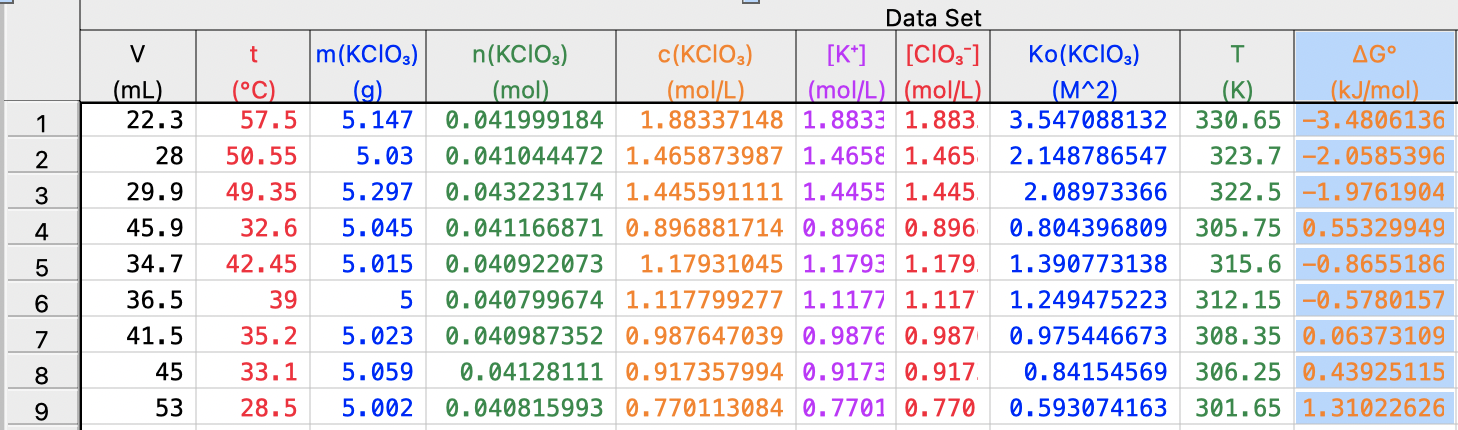
\includegraphics[width=\textwidth]{regneark.png}
\end{center}
\caption{Udregningerne er lavet i Logger Pro}
\label{fig:regneark}
\end{figure}
Siden vi fra ligning \ref{eq:GafT} (hvor $\Delta H \stst $ og $\Delta S \stst $ er konstante) har, at der er en lineær sammenhæng mellem $\Delta G \stst $ og $T$, laver vi en lineær regression, hvilket ses i \cref{fig:regression}.
\begin{figure}[H]
\begin{center}
  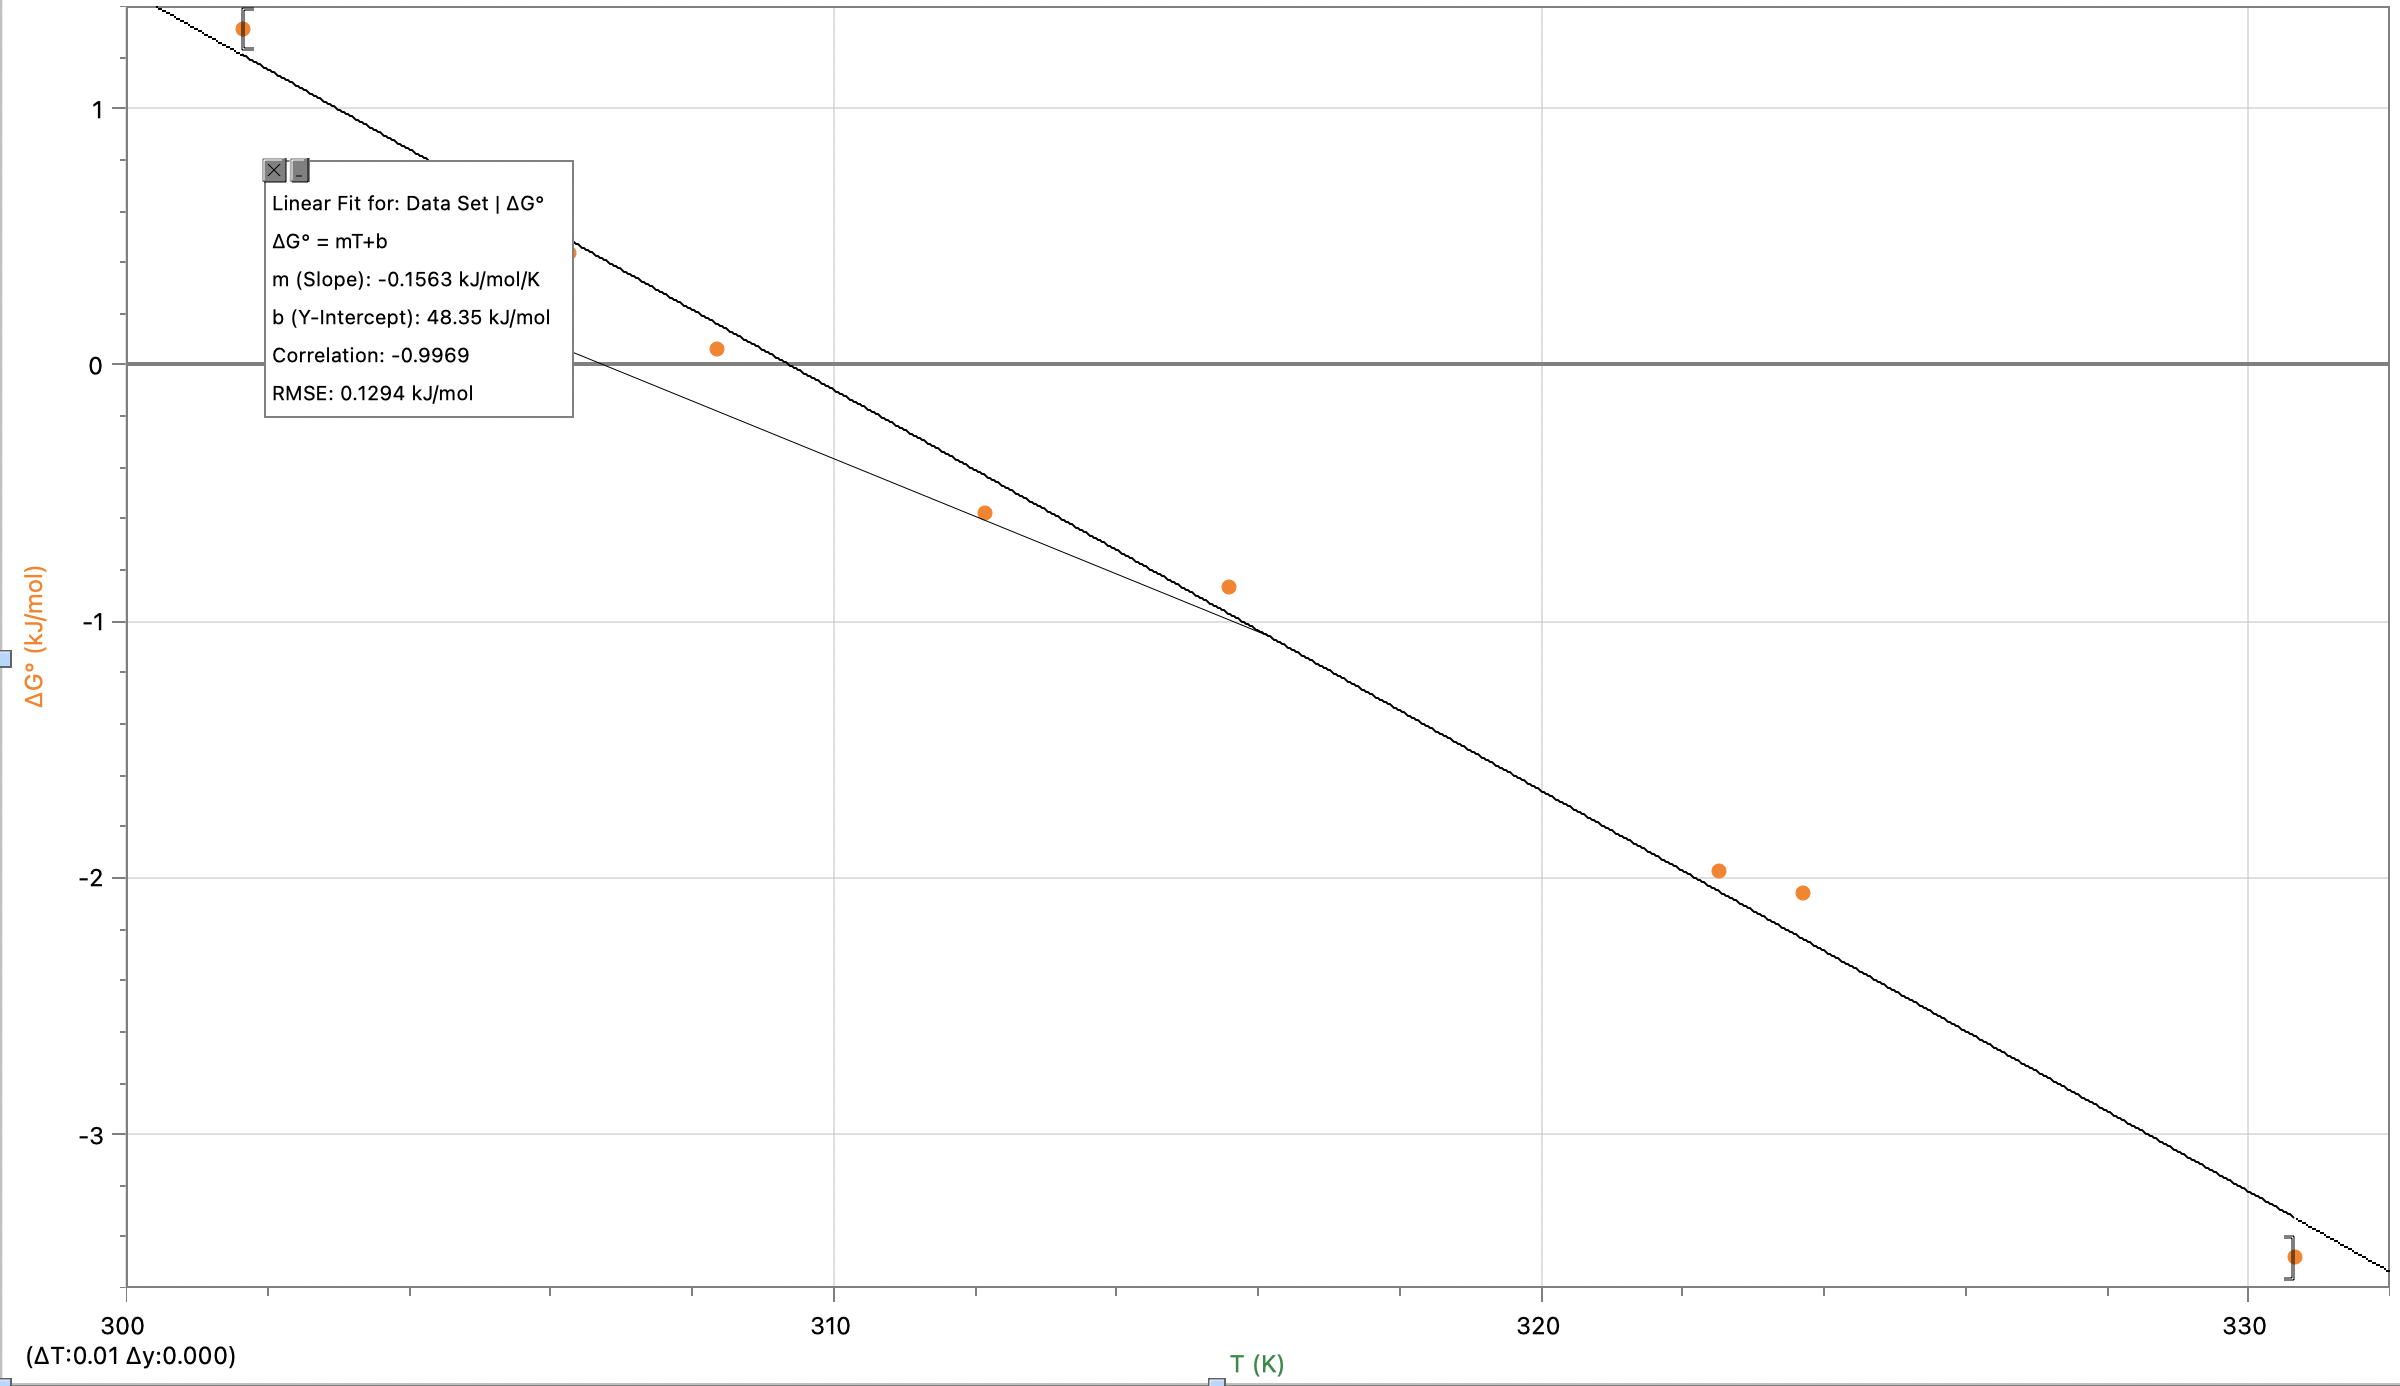
\includegraphics[width=\textwidth]{regression.png }
\end{center}
\caption{Lineær regression lavet i Logger Pro}
\label{fig:regression}
\end{figure}
Punkterne ligger tilnærmelsesvist på en ret linje, og vi har fra vores regression, at 
\[
\Delta G \stst =48,35 \;\unit{kJ/mol} -T \cdot 0,1563 \;\unit{\frac{kJ}{mol \cdot K}} 
\] 
Hvis vi kombinerer dette med ligning \ref{eq:GafT}, kan vi finde værdier for $\Delta H \stst $ og $\Delta S \stst $. 
\begin{equation*}
\begin{split}
  \Delta H \stst &=48,35 \;\unit{kJ/mol} \approx 48,4 \;\unit{kJ/mol} \\
  \Delta S \stst &=0,1563 \;\unit{\frac{kJ}{mol \cdot K}} \approx 156 \;\unit{\frac{J}{mol \cdot K}}
\end{split}
\end{equation*}
Vi ser da, at $\Delta H \stst > 0$, hvilket betyder, at reaktionen mod højre er endoterm.
Derudover er $\Delta S \stst > 0$, hvilket betyder, at uordenen forøges ved reaktionen mod højre.

Da $\Delta G \stst $ aftager, når temperaturen forøges, så stiger opløseligheden med temperaturen (fordi $\Delta G \stst <0$ for at kemisk reaktion kan forløbe spontant ved konstant tryk og temperatur).  
Dette er i overensstemmelse med Le Chateliers princip, da reaktionen mod højre jo er endoterm.

Vi er også interesserede i at beregne $\Delta G \stst $ ved $298 \;\unit{K} $, hvilket er cirka $25 \;\unit{\celsius} $.
\begin{equation*}
\begin{split}
  \Delta G \stst (298 \;\unit{K} )&=48,35 \;\unit{kJ/mol} -298 \;\unit{K} \cdot 0,1563 \;\unit{\frac{kJ}{mol \cdot K}} \\
  &\approx 1,77 \;\unit{kJ/mol} 
\end{split}
\end{equation*}
\section*{Mulige fejlkilder}
Ved forsøgene er det svært at bestemme præcist, hvornår kaliumchlorat begynder at udfælde sig igen, hvilket ville føre til en lavere målt temperatur, hvis man opdager udfældningen for sent.

\section*{Konklusion}
Vi har for reaktion \ref{eq:opløsning} bestemt $\Delta G \stst (298 \;\unit{K} )=1,77 \;\unit{kJ/mol} $, $\Delta H \stst =48,4 \;\unit{kJ/mol} $ og $\Delta S \stst =156 \;\unit{\frac{J}{mol \cdot K}} $. 
\end{document}
